\documentclass[helvetica]{seminar} 
\input{xy}
\xyoption{all}
\usepackage{graphicx} 
\usepackage{slidesec} 
% \usepackage{url}
\usepackage{hyperref}
\usepackage[framemethod=TikZ]{mdframed}
\usepackage{color}
\usepackage[normalem]{ulem}  

\def\dash---{\unskip\kern.16667em---\penalty\exhyphenpenalty\hskip.16667em\ignorespaces}
\long\def\symbolfootnote[#1]#2{\begingroup%
\def\thefootnote{\fnsymbol{footnote}}\footnote[#1]{#2}\endgroup}

% to fix problems making landscape seminar pdfs
% Letter...
\pdfpagewidth=11truein
\pdfpageheight=8.5truein
\pdfhorigin=1truein     % default value(?), but doesn't work without
\pdfvorigin=1truein     % default value(?), but doesn't work without
% A4
%\pdfpagewidth=297truemm % your milage may vary....
%\pdfpageheight=210truemm
%\pdfhorigin=1truein     % default value(?), but doesn't work without
%\pdfvorigin=1truein     % default value(?), but doesn't work without


\renewcommand{\familydefault}{\sfdefault}  
 
\input{seminar.bug} 
\input{seminar.bg2} % See the Seminar bugs list 
 
\slideframe{none} 
 
 
\usepackage{fancyhdr} 
 
% Headers and footers personalization using the `fancyhdr' package 
\fancyhf{} % Clear all fields 
\renewcommand{\headrulewidth}{0mm} 
\renewcommand{\footrulewidth}{0.1mm} 
 
\fancyfoot[L]{\tiny IETF 101} 
\fancyfoot[C]{\tiny IASA 2.0}
\fancyfoot[R]{\tiny \theslide} 
 
 
% To center horizontally the headers and footers (see seminar.bug) 
\renewcommand{\headwidth}{\textwidth} 

% To adjust the frame length to the header and footer ones 
\autoslidemarginstrue 
\pagestyle{fancy} 
 

\newcommand{\heading}[1]{% 
  \begin{center} 
    \large\bf 
    #1 
  \end{center} 
  \vspace{.4 in}} 



\begin{document}

\begin{slide}
\begin{center}
\vspace{.5 in}
\LARGE{{\bf}IASA 2.0 Legal Options \& Strawman\\{\small Morgan Lewis Memo / \verb^draft-hall-iasa20-struct-01^}}\\
\vspace{.2in}
\large{
\begin{tabular}{ c c c }
J.L. Hall  & J. Arkko & L. Daigle \\
B. Haberman & J. Livingood  & E. Rescorla 
\end{tabular}
}
\end{center}
\end{slide}

\centerslidesfalse 


\begin{slide}

\heading{IASA 2.0 Work So Far}

{\footnotesize
  \vspace{-8ex}
\begin{itemize}
\item IETF Chairs began process to explore
  \href{https://mailarchive.ietf.org/arch/msg/ietf/NBhbbeFr-UZq86YnjUn2XKEEDUk}{updating
    IASA} (Feb-2017)
\item Some thoughts on existing structure were documented:
  \begin{itemize}
  \item \href{https://tools.ietf.org/html/draft-daigle-iasa-retrospective-01}{draft-daigle-iasa-retrospective}, \href{https://tools.ietf.org/html/draft-arkko-ietf-iasa-thoughts-00}{draft-arkko-ietf-iasa-thoughts}, \href{https://tools.ietf.org/html/draft-arkko-ietf-finance-thoughts-00}{draft-arkko-ietf-finance-thoughts}
  \end{itemize}
\item Design Team recruited: (Arkko, Daigle, Haberman, Hall,
  Livingood, Rescorla)
\item Two virtual workshops and DT recommendations:
  \begin{itemize}
  \item ``Report from the IASA 2.0 Virtual
    Workshops''\\ \href{https://tools.ietf.org/html/draft-hall-iasa20-workshops-report-00}{draft-hall-iasa20-workshops-report}
  \item ``IASA 2.0 Design Team
    Recommendations''\\ \href{https://tools.ietf.org/html/draft-haberman-iasa20dt-recs-01}{draft-haberman-iasa20dt-recs}
  \end{itemize}
\item After Singapore, we ruled out complete independence, community
  asked for clarilty on organizational structure:
  \begin{itemize}
  \item Memorandum from ISOC tax lawyers:
    \href{https://mailarchive.ietf.org/arch/msg/iasa20/XT_3vfd3OWVFCW335mRrvWuusaI/}{Morgan
      Lewis Memo}
  \item A Strawman design of an IASA 2.0:
    \href{https://datatracker.ietf.org/doc/draft-hall-iasa2-struct/}{draft-hall-iasa2-struct}
  \end{itemize}
\end{itemize}
}
\end{slide}

%% \begin{slide}

%%   \begin{center}
%%     \resizebox{6.5cm}{!}{
%%       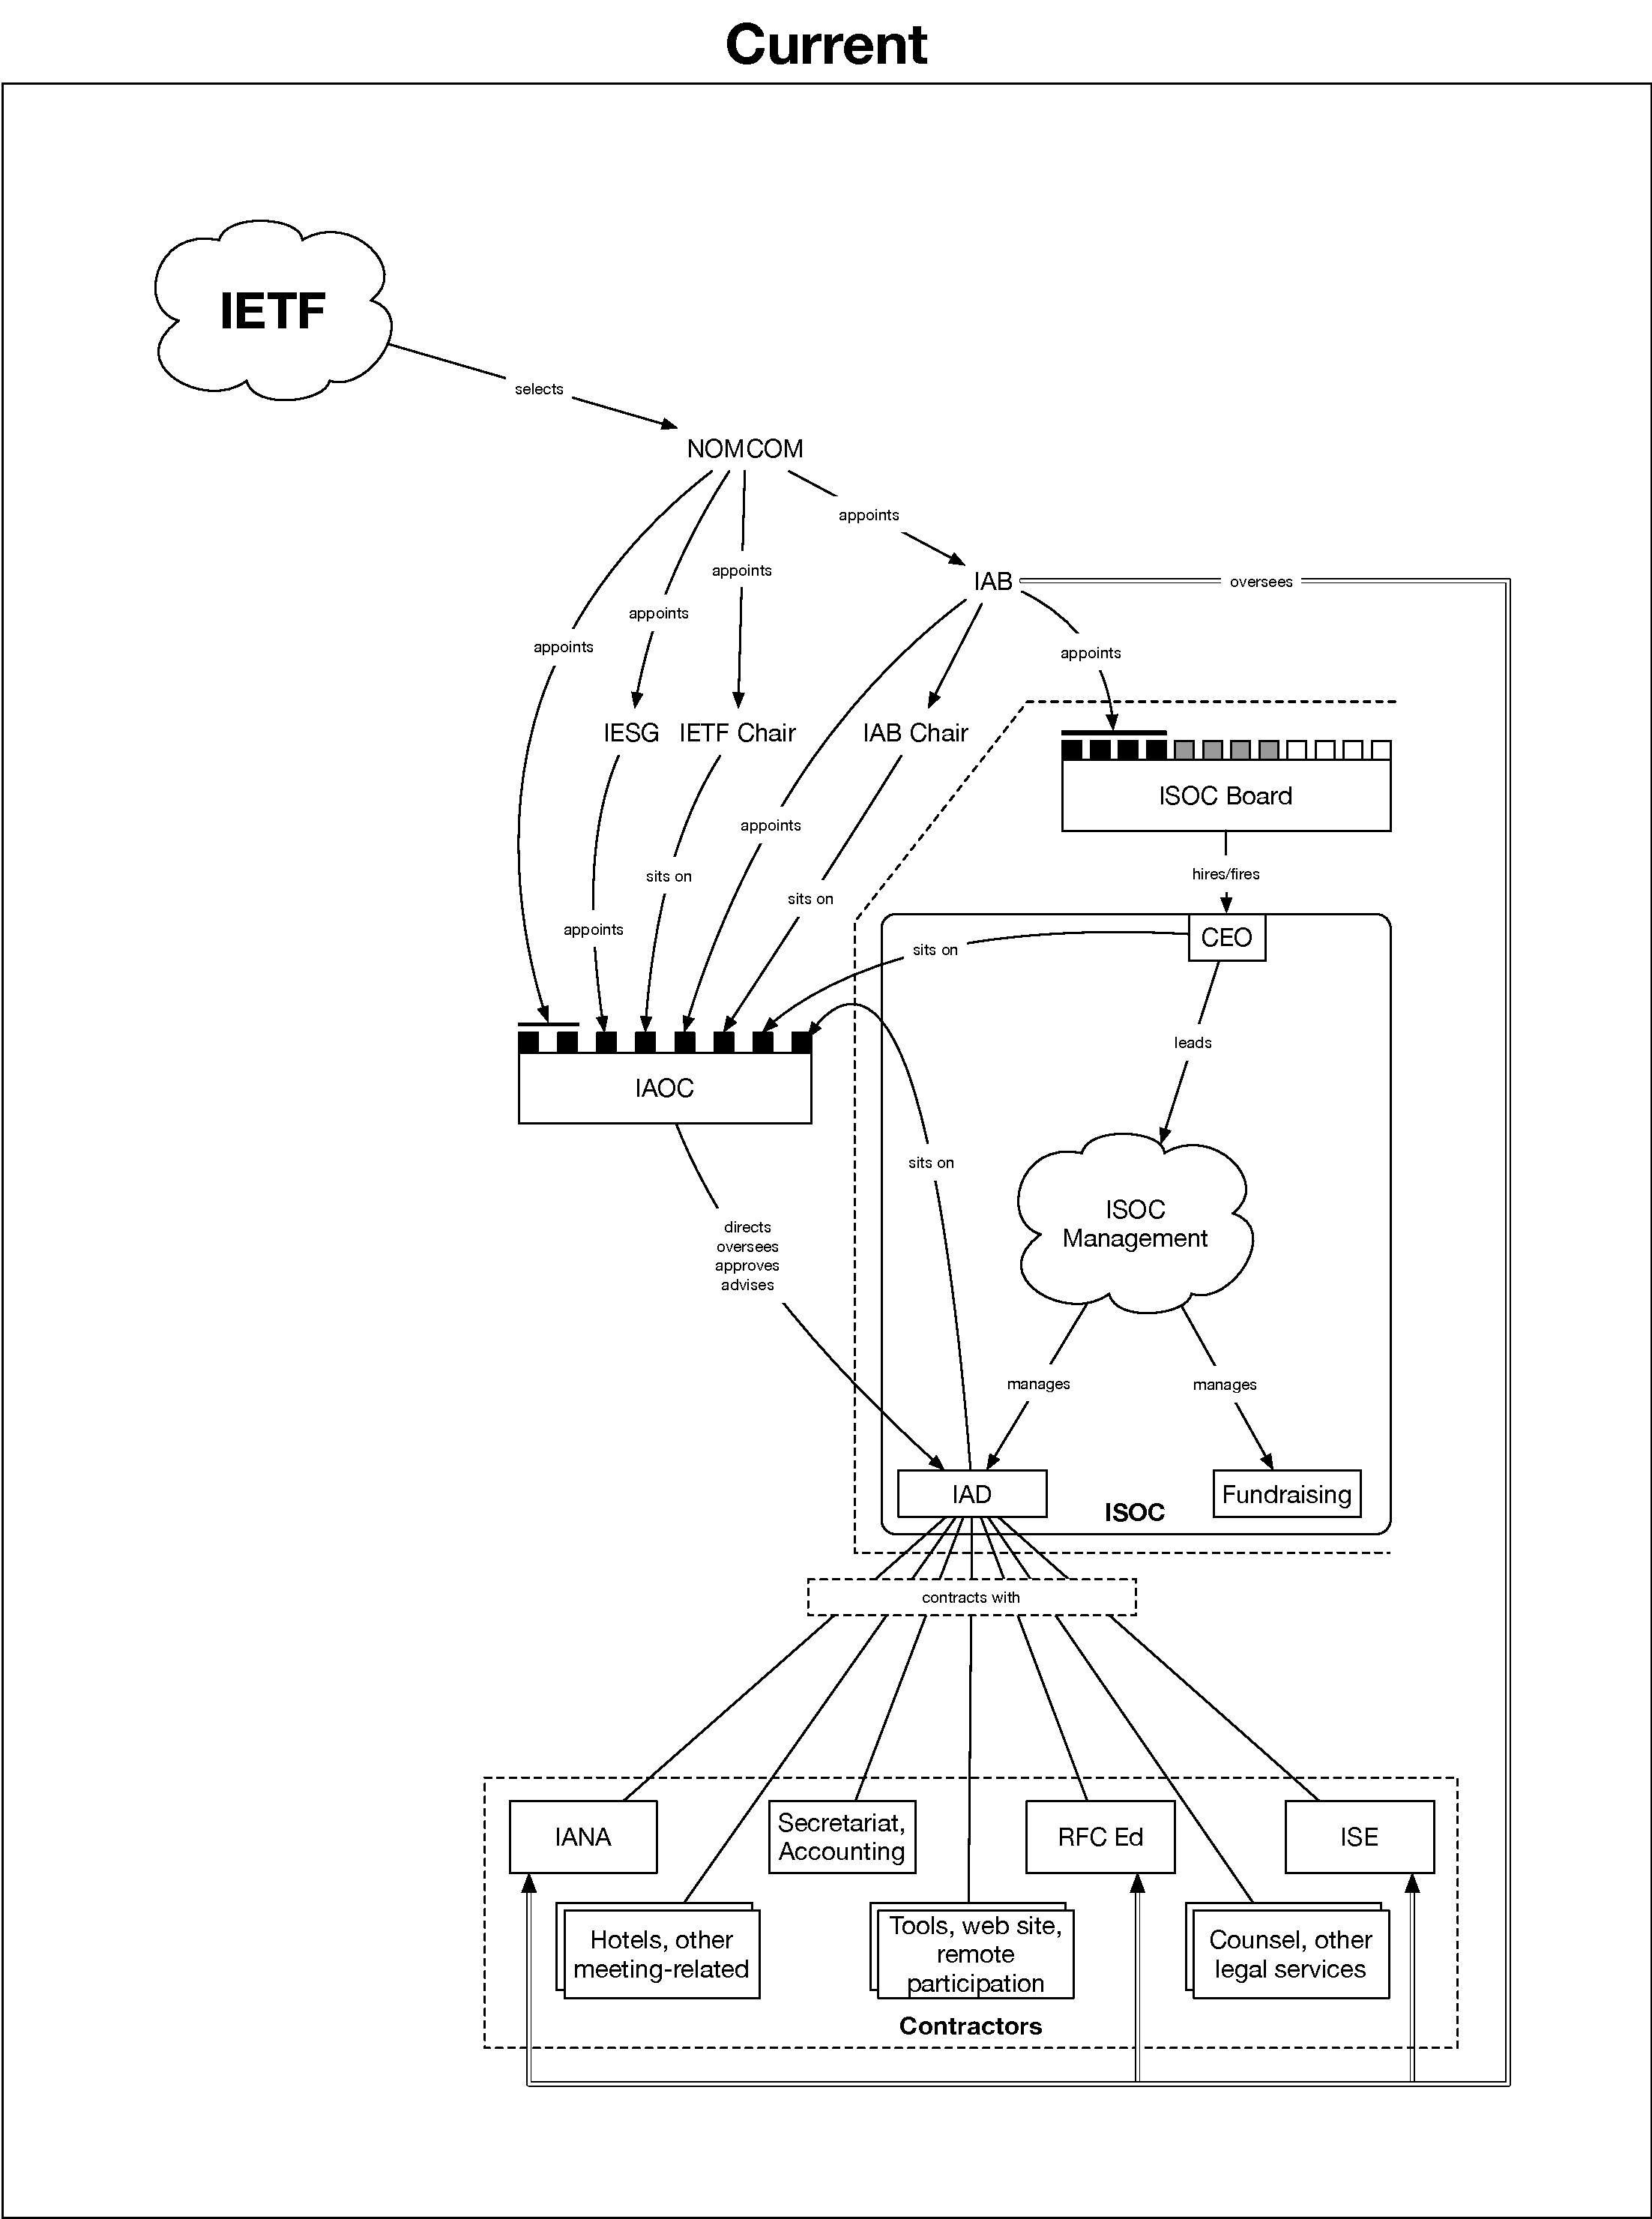
\includegraphics{current.pdf}
%%     }
%%   \end{center}

%% \end{slide}

%% \begin{slide}

%%   \begin{center}
%%     \resizebox{6.5cm}{!}{
%%       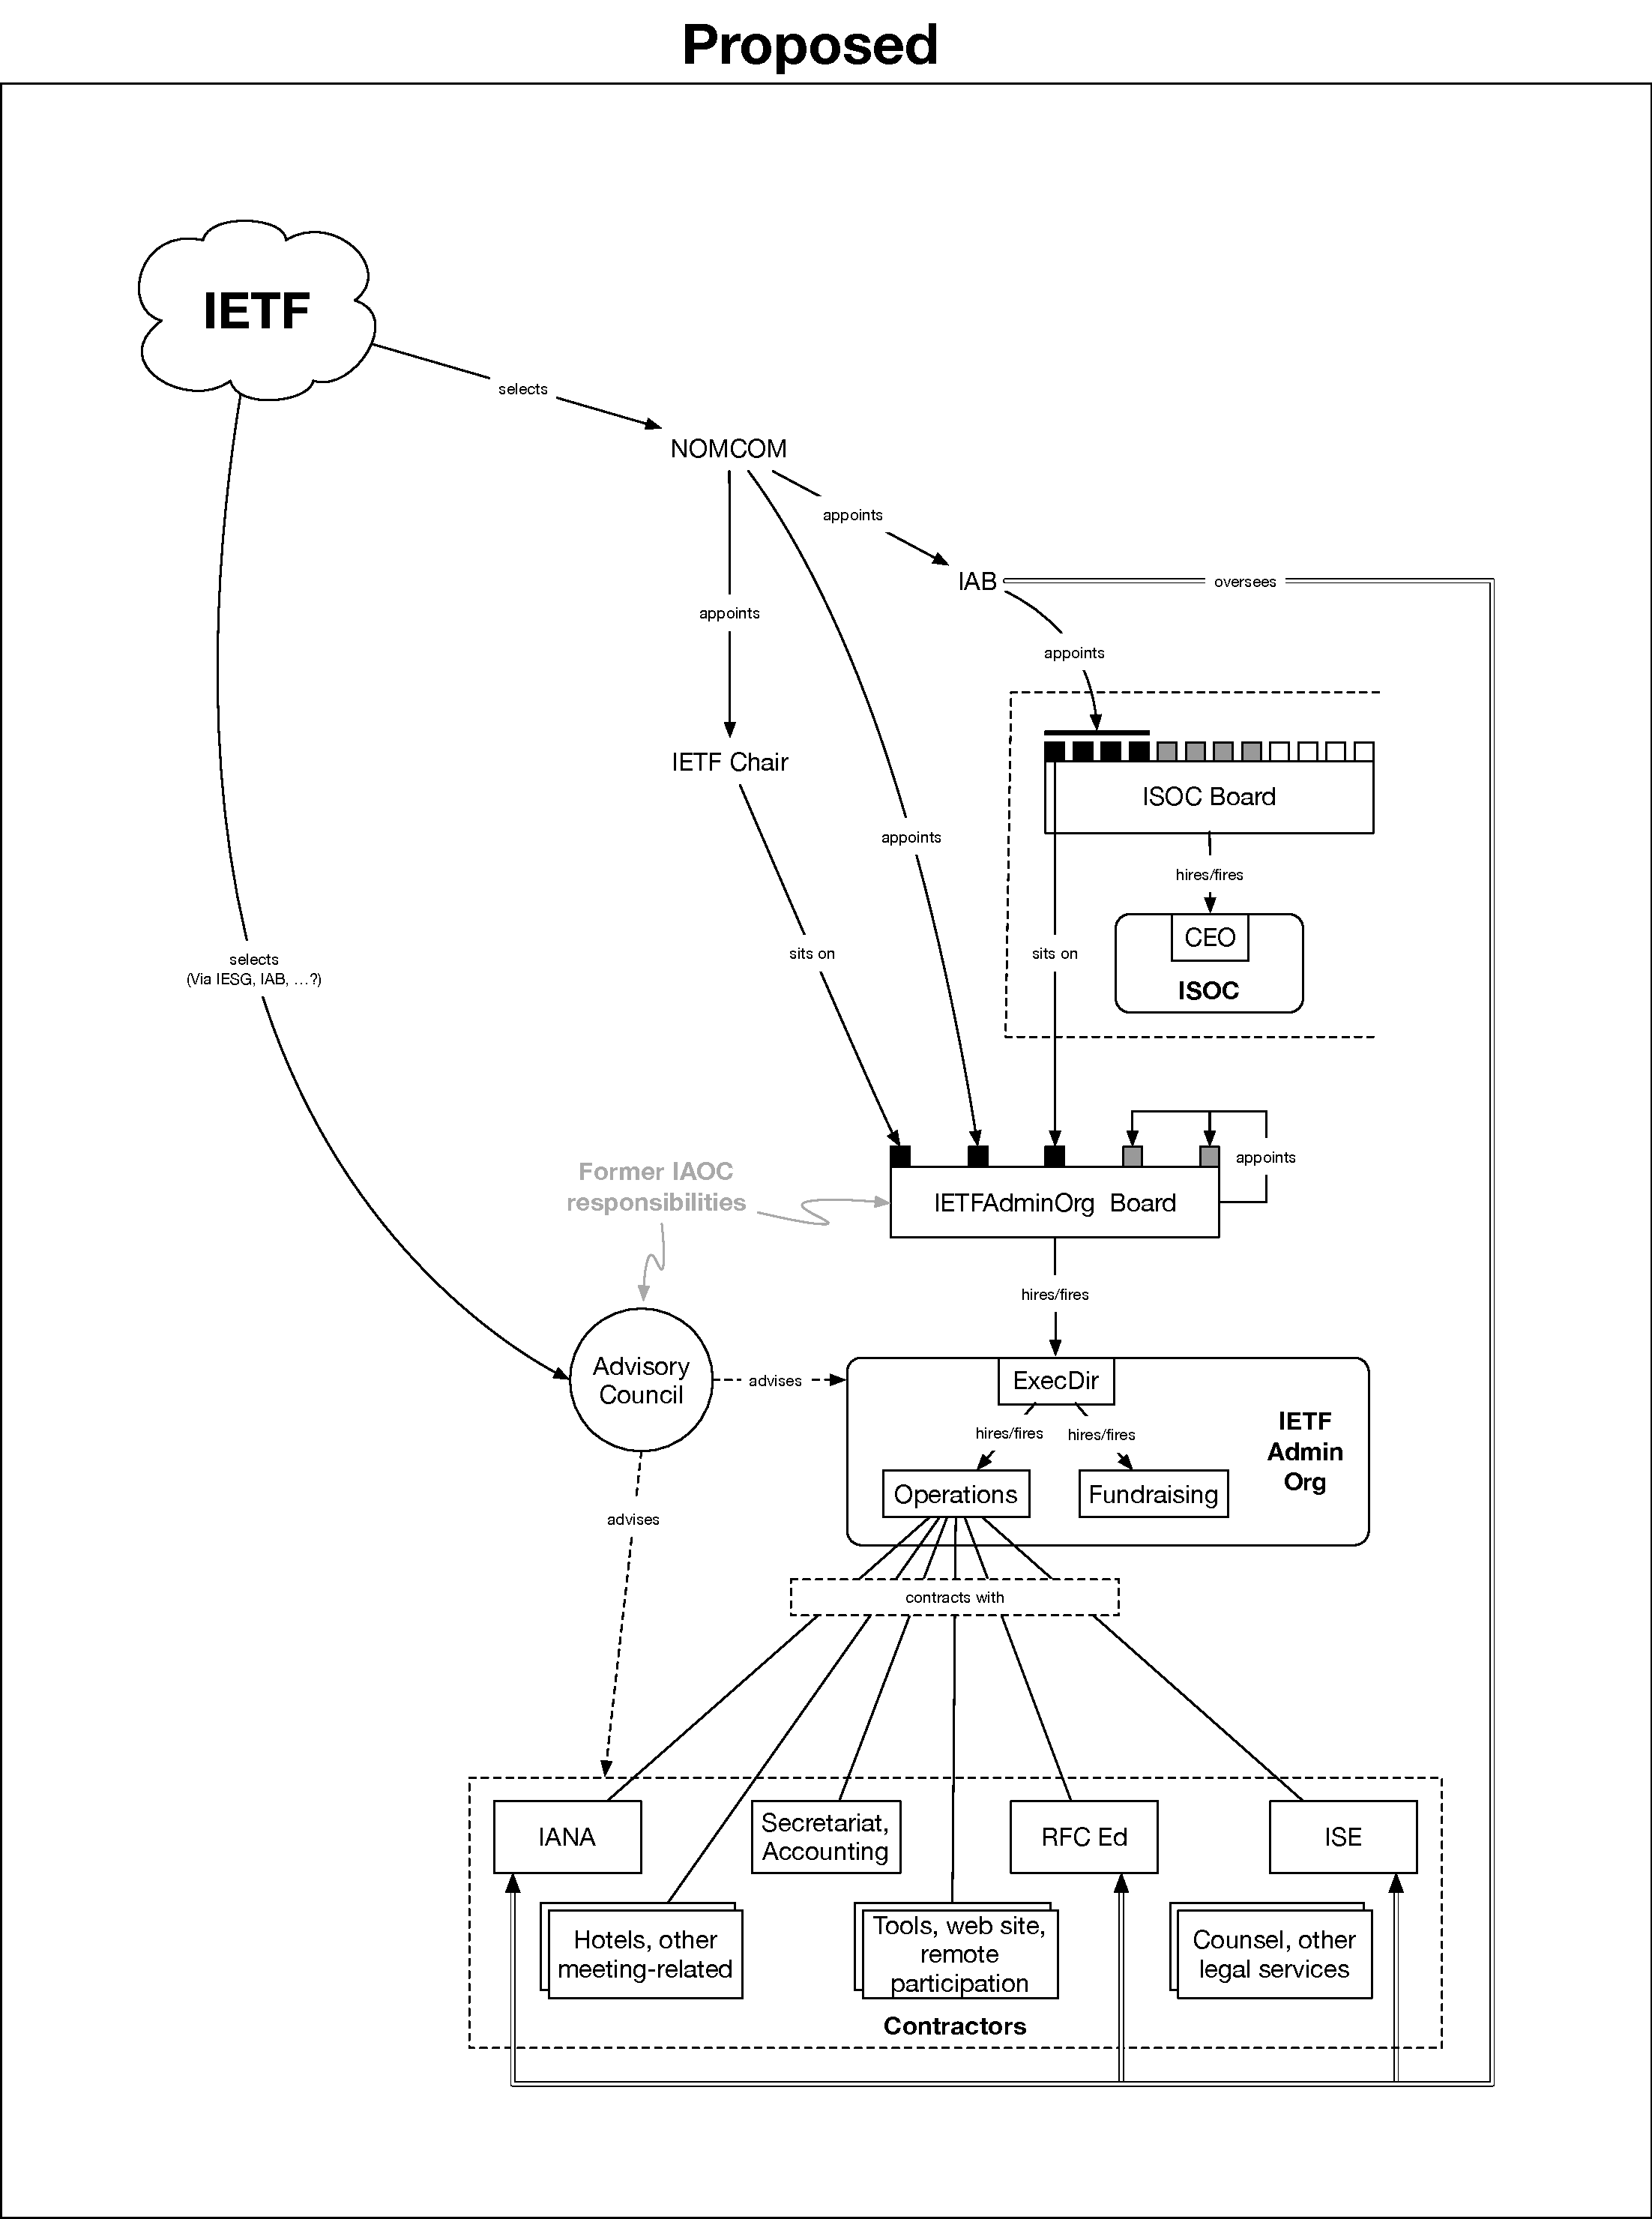
\includegraphics{proposed.pdf}
%%     }
%%   \end{center}

%% \end{slide}

%% \begin{slide}

%%   \begin{center}
%%     \resizebox{6.5cm}{!}{
%%       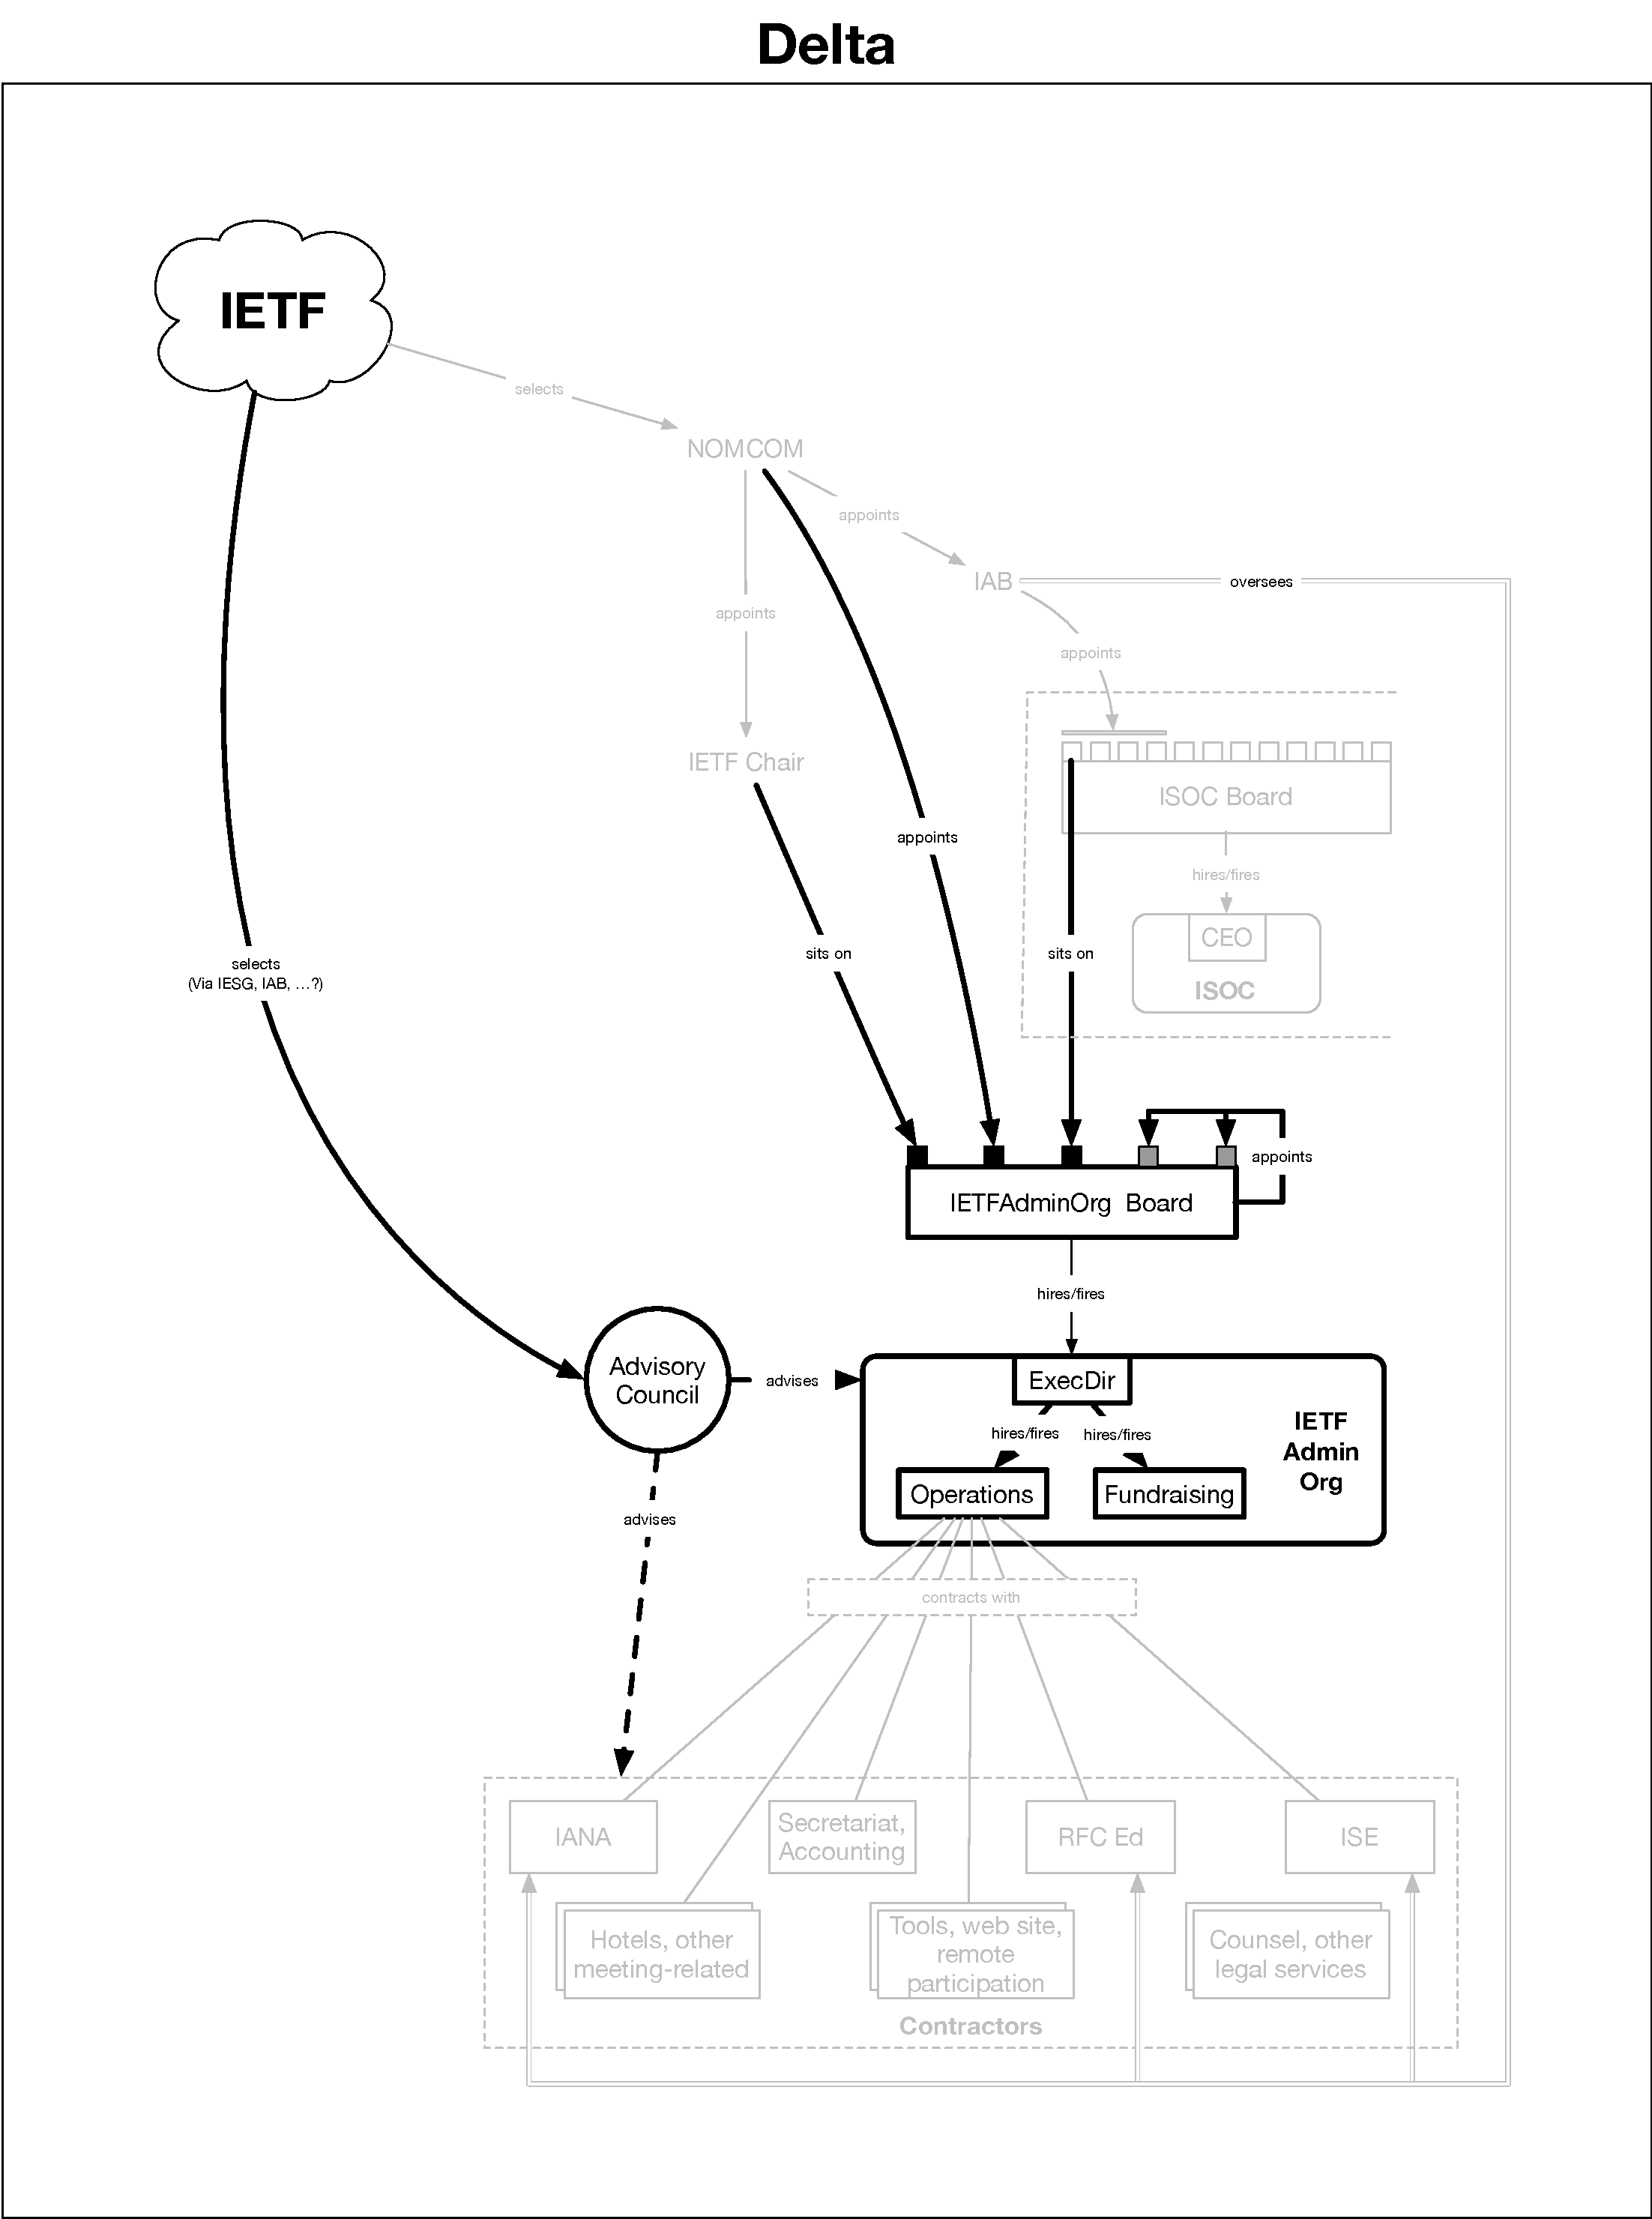
\includegraphics{delta.pdf}
%%     }
%%   \end{center}

%% \end{slide}

\begin{slide}
\resizebox{11cm}{!}{
%\vspace{-8ex}         %for long lists
%\hspace{-1.5cm}         %move left
{\tiny
\begin{centering}         
\begin{tabular}{ | p{2.0cm} | p{0.8cm} | p{1.9cm} | p{2.6cm} | p{1.0cm} |}
  \hline
  \href{https://tools.ietf.org/html/draft-haberman-iasa20dt-recs-01}{\textbf{draft-haberman:}} & \multicolumn{1}{|c|}{independent} & \multicolumn{2}{|c|}{ISOC Subsidiary} & \multicolumn{1}{|c|}{IASA++} \\ \hline
  \href{https://mailarchive.ietf.org/arch/msg/iasa20/XT_3vfd3OWVFCW335mRrvWuusaI/}{\textbf{Morgan Lewis memo:}} & \multicolumn{1}{|c|}{independent} & \multicolumn{1}{|c|}{Type-I support org} & \multicolumn{1}{|c|}{LLC} & \multicolumn{1}{|c|}{Activity of ISOC} \\ \hline \hline
  \multicolumn{5}{|c|}{\textbf{I. Governance}} \\ \hline
  Would ISOC be required to be involved in appointing board members of IETFAdminOrg (IAO)? & No & Yes. ISOC to appoint majority of IAO Board members, perhaps upon IETF recommendations. & No. ISOC can delegate responsibility for appointing all IAO Board members to IETF bodies, but retain ultimate control of the LLC & Yes, as \mbox{today} \\ \hline
  Can IAO Board hire and fire the IAO Exec Dir? & Yes & Yes & Yes & No \\ \hline
  Is ISOC liable for IAO's debts and obligations? & No & No & No & Yes \\ \hline
  \multicolumn{5}{|c|}{\textbf{II. Finance \& Fundraising}} \\ \hline
  Can IETF funds be held in a bank account separate from ISOC funds? & Yes & Yes & Yes & Yes \\ \hline
  Can donors write checks to IAO? & Yes & Yes & Yes & No \\ \hline
  Would IAO need to maintain its own non-profit status? & Yes & Yes & No & No \\ \hline
   \multicolumn{5}{|c|}{\textbf{III. Administrative Complexities}} \\ \hline
  Would IAO need to conduct its own audit & Yes & Yes & No & No \\ \hline
  Would IAO need to file its own form 990? & Yes & Yes & No & No \\ \hline
  \multicolumn{5}{|c|}{\textbf{IV. Staffing}} \\ \hline
  Can IAO Exec Dir hire and fire staff and contractors without ISOC approval? & Yes & Yes & Yes & No \\ \hline
\end{tabular}
\end{centering}
}
}
\end{slide}


\begin{slide}

\heading{draft-hall-iasa20-struct-01}

\begin{itemize}
\item An attempt at a proposed structure, far from perfect
\item Points of discussion on the \texttt{iasa20} list:
  \begin{itemize}
  \item Transparency of IAO and IAO Board
    \begin{itemize}
    \item Can we agree to something like this?:\\\textbf{``Whatever
      doesn't have a specific justification for being kept
      confidential, should be made public.  There must exist a public
      list of confidential items, describing the nature of the
      information and the reason for confidentiality.''} (need to take
      to IETF community)
    \end{itemize}
  \end{itemize}
\end{itemize}

\end{slide}



\begin{slide}

\heading{draft-hall-iasa20-struct-01}

\begin{itemize}
\item Points of discussion on the \texttt{iasa20} list (cont'd.):
  \begin{itemize}
  \item Board size, composition, compensation
    \begin{itemize}
    \item Size: 5 (too small?), maybe 7 (where to add?)
    \item draft-hall (5): IETF~Chair, 1 ISOC~Board (IAB-appointed), 1
      NOMCOM-appointed, 2 Members selected by IAO Board
    \item Ted H. (10): IETF~Chair, 5 ISOC~Board (IAB-appointed), 3
      NOMCOM-appointed, and IAO ED (\textit{ex oficio})
    \item Compensation? Term lengths? Staggered? Management/Finance
      Experience? Liasons? Officers?
    \end{itemize}
  \end{itemize}
\end{itemize}

\end{slide}



\begin{slide}

\heading{draft-hall-iasa20-struct-01}

\begin{itemize}
\item Points of discussion on the \texttt{iasa20} list (cont'd.):
  \begin{itemize}
  \item Advisory Council function, existence
    \begin{itemize}
    \item Proposed to offer community guidance to IASA and IAO~ED.
    \item Function like IAOC committees do today, but purely advisory.
    \item Size, composition, rhythyms, and requirements unclear.
    \item M. Richardson: can't we just spin up WGs for this?
    \end{itemize}
  \end{itemize}
\end{itemize}

\end{slide}


\begin{slide}

\heading{draft-hall-iasa20-struct-01}

\begin{itemize}
\item Points of discussion on the \texttt{iasa20} list (cont'd.):
  \begin{itemize}
  \item What about options in non-US jurisdictions?
    \begin{itemize}
    \item ML attorneys recommend against: taxpayers in U.S. could not
      take a charitable deduction; potential limitations of ISOC
      financial support; may need to apply for tax exemption/follow
      laws of $\geq2$ countries.
    \item M. Richardson: Do any options make it easier for non-US
      donations?
    \end{itemize}
  \end{itemize}
\end{itemize}

\end{slide}



\end{document} 

                
